\documentclass[dvipdfmx]{jsarticle}
\usepackage{graphics}
\usepackage{amsmath}
\usepackage{amssymb}
\usepackage{amsthm}
\usepackage{mathtools}
\usepackage{ascmac}
\usepackage{bm}
\usepackage{url}
\usepackage{txfonts}
\usepackage{color}
\usepackage{tikz}
\usetikzlibrary{calc}
\usetikzlibrary{intersections}

\begin{document}
    \section*{初めに}
    中学数学の中でのやや面倒な単元である濃度と密度について扱う.この2つは根元のところで同じなので,同時に理解したい.この資料は中学生向けではある.しかし,読みにくい場合は両親の助けを借りるように.

    さて,早速だがこの資料で一番大事なテーマをここで示しておく.それは

    {\centering 一部分がわかれば全体の様子がわかる\\}
    というものだ.
    これは科学(理系の勉強)のすべてに共通する大事な発想だ.濃度・密度は一部分を知ることで全体がわかる最も簡単な例になっている.


    次の節から本題に入る.まずは濃度から扱う.

    \section{濃度}
    \subsection{同じしょっぱさ}
    食塩水の濃度を考える問題では,外すことができない大事な条件がある.問題文には書かれていないことが多い.それは,"食塩水は完全に混ざっている"という条件だ.簡単に言うと,食塩水のどの部分を飲んでも同じしょっぱさだということだ.そして,それは大きな食塩水のバケツからいくらコップに食塩水をくんできても同じものになるということでもある(図\ref{tikz_baketu_shokuensui}).

    \begin{figure}[htbp]\centering
        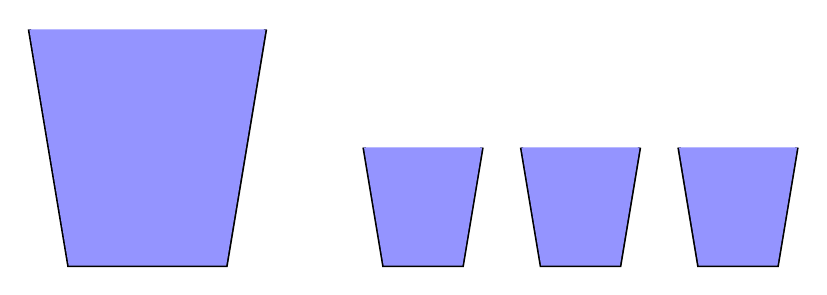
\begin{tikzpicture}\large
            \draw[very thick]($2*(-.25,1.5)$)--(0,0)--($2*(1,0)$)--($2*(1.25,1.5)$);
            \fill[blue!42]($2*(-.25,1.5)$)--(0,0)--($2*(1,0)$)--($2*(1.25,1.5)$);

            \foreach \x in{4,6,8}{
                \draw[very thick](\x -.25,1.5)--(\x,0)--(\x +1,0)--(\x +1.25,1.5);
                \fill[blue!42](\x -.25,1.5)--(\x,0)--(\x +1,0)--(\x +1.25,1.5);
            }

        \end{tikzpicture}
        \caption{大きなバケツから食塩水をとる}
        \label{tikz_baketu_shokuensui}
    \end{figure}

    間違っても図\ref{tikz_baketu_shokuensui_sub}のように,くんだコップによってしょっぱい度合いが変わることはない.

    \begin{figure}[htbp]\centering
        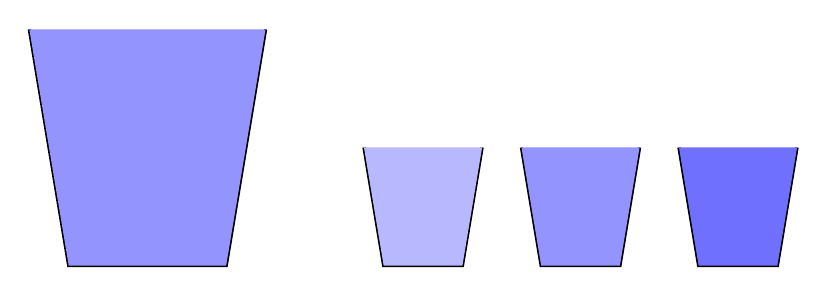
\begin{tikzpicture}\large
            \draw[very thick]($2*(-.25,1.5)$)--(0,0)--($2*(1,0)$)--($2*(1.25,1.5)$);
            \fill[blue!42]($2*(-.25,1.5)$)--(0,0)--($2*(1,0)$)--($2*(1.25,1.5)$);

            \foreach \x in{28,42,56}{
            \draw[very thick](\x/7 -.25,1.5)--(\x/7,0)--(\x/7 +1,0)--(\x/7 +1.25,1.5);
            \fill[blue!\x](\x/7 -.25,1.5)--(\x/7,0)--(\x/7 +1,0)--(\x/7 +1.25,1.5);
            }

        \end{tikzpicture}
        \caption{大きなバケツから食塩水をとる}
        \label{tikz_baketu_shokuensui_sub}
    \end{figure}

    この条件は,コップの様子を知ることができれば,バケツ全体の様子がわかることを示している.つまり,"一部分がわかれば全体のようすがわかる"である.

    \subsection{コップとバケツ}
    前項\footnote{この資料では「濃度」や「同じしょっぱさ」という部分に番号が振ってある.これは節・項を示している.「濃度」節の「同じしょっぱさ」項と理解しよう.つまり,ここでの前項は「同じしょっぱさ」項である.このような書き方は以降も続く.}でバケツの水をコップに取り出すと,コップにバケツの様子が部分として現れることを述べた.これをもっと数学的に考える.

    数学的というのはコップというまちまちな基準\footnote{どんなコップでもいいというのは,数学的ではない.}ではなく,1つの変化しない基準を使うということだ.そこで使うのが \(1\ \mathrm{g}\)という重さだ.当然,この重さは変化しない.
    そして, \(1\ \mathrm{g}\)というコップに対して,バケツに当たるのが水溶液全体の重さ(g)ということになる.

    ここまでで,何となくコップとバケツが数学的に何になるのかがわかったが,いまいち関係がつかめない.これは水溶液の様子というのが何なのかを示していないからだ.これは次項で述べる.

    \subsection{水溶液の様子}
    これまでの話で,水溶液の"様子"というのは全体を示すバケツからだけではなく,その一部分のコップからもわかることを述べた.
    さらに,バケツは水溶液全体のことを意味していて,コップが一部分を意味していると説明した.
    ここでは水溶液の"様子"というものが何なのかを明らかにする.

    結論から述べると,水溶液の"様子"というのは,
    水溶液に溶ける溶質(塩など)の重さ[\(\mathrm{g}\)]のことだ.水溶液を扱う問題で理解が難しいのは,この水溶液の"様子"というものと,"濃度"というものに区別をつけることである.
    区別は次のようになっている(図\ref{tikz_yosu_nodo}).

    \begin{figure}[htbp]\centering
        \begin{tikzpicture}
            \node[draw](a) at (0,0){\(1\ \mathrm{g}\)の水溶液中の塩の重さ:濃度};
            \node[draw](b) at (7,0){全体の塩の量:様子};
            \draw[thick,<->](a)node[above=3mm]{一部分}--node[above]{食塩水の重さ(g)}(b)node[above=3mm]{全体};
        \end{tikzpicture}
        \caption{"様子"と"濃度"}
        \label{tikz_yosu_nodo}
    \end{figure}

    この関係がわかっていると実際に濃度を計算するときの式に間違いが起きにくい.

    \subsection{濃度の計算}
    ここまでの話を使って,ようやくここで濃度を計算する.
    % 水溶液の濃度を考えるときは食塩水の量や水の量,塩の量はすべてグラムで考える.
    まず図\ref{tikz_baketu_shokuensui}のように全体の水溶液から \(1\ \mathrm{{g}}\)ずつ水溶液を分けてゆくことをイメージする.このとき,コップのしょっぱさはすべて同じなのだから, \(1\ \mathrm{g}\)のコップに入っている塩の重さはすべて同じといえる\footnote{同じ重さの食塩水で同じしょっぱさなら,塩の重さは同じに決まっている.}.つまり,塩だけに注目するとバケツからコップに分けるとは,塩を同じ重さで分けるということになる.

    元のバケツをすべてコップに分けると,塩はすべてのコップに同じ重さずつ入ることになる\footnote{ピッタリいかない最後のコップは仕方ない.}.では1つのコップにどれだけの重さ塩が入るかは,元の全体の塩の重さをコップの数\footnote{コップの数は水溶液の重さそのものである.}で割ればいいことがわかる.

    % 元の塩の量はすぐにわかる.さらにコップの数は,バケツに入った食塩水の量であるとわかる.ここから次の式を与えることができる.

    最後に濃度は百分率で表さなければならないので100をかける\footnote{これについては次項で述べる.}ことを忘れなければ,次の式を立てることができる.

    \begin{equation}
        (\text{食塩水の濃度(\%)}) = \frac{(\text{塩の重さ(g)})}{(\text{食塩水の重さ(g)})}\times 100
    \end{equation}

    食塩水の重さは食塩水の作るときに使う塩の重さと,水の重さの和ということができるので,次のようにすることもできる.

    \begin{equation}
        (\text{食塩水の濃度(\%)}) = \frac{(\text{塩の重さ(g)})}{(\text{水の重さ(g)})+(\text{塩の重さ(g)})}\times 100
    \end{equation}

    % 基本的に水溶液の濃度の計算では塩が変わったりすることがあっても上の2つの式を使うだけでよい.

    \subsection{百分率}
    百分率とは,小さな数値に100かけることで見やすい値にする計算方法だ.小さな数値というのも特に0から1までの範囲に入る数値のことだ.それ以上の意味があるわけではない.

    例えば,コインの裏表は2分の1の確率で \(1/2=0.5\)であるが,百分率では
    \[
    0.5\times 100 =50\ \%
    \]
    となる.

    これを濃度でも使う.
    \[
    \frac{(\text{塩の重さ(g)})}{(\text{食塩水の重さ(g)})}
    \]
    この値は確実に0から1までの間に入る数\footnote{食塩水の重さは必ず塩の重さより大きい.}なので100をかけて見やすくすることで濃度とする.

    \section{濃度計算の理解}
    ここまでで,水溶液の成り立ちや公式について述べた.ここでそれらをまとめる.
    \subsection{目的}
    まずは濃度を利用する目的だ.もともとの目的はバケツの中にある水溶液に入っている塩の量を求めることだ.これを達成するために,バケツの中身をすべて出していては無駄が多い.そのため,コップ1杯の水溶液に注目して計算することで,塩の量を求めるのだ.

    このとき,水溶液の塩がまんべんなく混ざっていることが,計算をするための条件となっていることに注意しよう.

    \subsection{計算方法}
    バケツの塩をコップに等分するというのが濃度の計算の最も大事な考え方だ.そして,コップというのが \(1\mathrm{g}\)であると考えることで計算が可能になる.バケツの中の水溶液を \(1\mathrm{g}\)のコップに分けるのだから,コップの数は
    \[
       (\text{コップの数})= \frac{\text{(バケツの中の重さ(g))}}{\text{(コップ1杯(g))}}=(\text{バケツの中の重さ(g)})
    \]
    ということになるので,コップ1杯当たりの塩の重さは
    \[
        (\text{コップ1杯の塩の重さ(g)})= \frac{(\text{塩の重さ})}{(\text{バケツの中の重さ(g)})}
    \]
    となる.

    ここまでで濃度といっても問題がないように感じるが,計算結果は必ず0から1の間の小さな数字になってしまう.これでは,どれくらい塩が入っているのかがわかりにくい.そこで100をかけることで百分率として見やすくするのだ.最終的に,濃度の計算は次の式でなされる.
    \begin{equation}
        (\text{濃度(\%)})=\frac{(\text{塩の重さ(g)})}{(\text{水溶液全体の重さ(g)})}\times 100=\frac{(\text{塩の重さ(g)})}{(\text{水の重さ(g)})+(\text{塩の重さ(g)})}\times 100
        \label{eq_concentration}
    \end{equation}

    濃度の計算で大事なのは全体であるバケツに入った塩の量と,一部分であるコップの中の塩の量だ.そして,コップの中にある塩の量が濃度であることを理解すれば,濃度の計算はいつでもできる.

    \section{密度}
    濃度のときに大事なテーマとなった"一部分がわかれば全体の様子がわかる"を密度にも応用する.密度を扱う問題で全体に当たるのは物体の重さで,一部分に当たるのは1 \(\mathrm{cm}^3\)あたりの重さであることをここで明らかにして,話を進めることにする.

    \subsection{同じ重さ}
    物体の密度を考える問題では濃度のときと同じで大事な条件がある.それは,物体のどの部分を切り出しても同じ大きさであれば,同じ重さであるということである.これは食塩水のときの,同じしょっぱさだということと共通する条件だ.このおかげで,物体の一部分の重さがわかることで全体の重さを知ることができる.

    \begin{figure}[htbp]\centering
        \begin{tikzpicture}
            \node[draw](a) at (0,0){\(1\ \mathrm{cm}^3\)の重さ:密度};
            \node[draw](b) at (7,0){物体の重さ:様子};
            \draw[thick,<->](a)node[above=3mm]{一部分}--node[above]{物体の大きさ (\(\mathrm{cm^3}\))}(b)node[above=3mm]{全体};
        \end{tikzpicture}
        \caption{"様子"と"密度"}
        \label{tikz_density_image}
    \end{figure}


    \subsection{物体のかけら}
    大きな物体の重さを考えるとき,その一部のかけらの重さによって全体の重さを考えることがある.これが密度だ.密度を考えるときは食塩水のコップと同じように一部分を用意しなければならない.密度はその一部分を1 \(\mathrm{cm}^3\)の大きさのかけらとすることにしている.この重さがわかれば,全体の大きさを知ることで重さまでわかるということになる.

    \subsection{密度の計算}
    以上の話から,十分に密度の計算ができる.密度は全体の重さをすべて1 \(\mathrm{cm}^3\)の一部分に分けるのだから,次の式になる.

    \begin{equation}
        (\text{密度}(\mathrm{g}/\mathrm{cm}^3)) = \frac{(\text{全体の重さ(g)})}{(\text{全体の大きさ}(\mathrm{cm}^3))}
        \label{eq_density}
    \end{equation}

    濃度と異なるのは最後に100をかけていない点だ.これに関しては濃度と密度の単位などが関係するので後で述べる.

    密度の計算で大事なのは全体のバケツに当たるものが物体の重さであり,一部分のコップに当たるのが \(1\ \mathrm{cm}^3\)のかけらの重さであるということだ.そして,密度というのが一部分の重さを表していることを理解していればいつでも密度の公式は思いつく.


    \section{濃度と密度の違い}
    全体の様子を知るために一部分に分けて考えるということは濃度と密度に共通する大事な特徴である.しかし,当然だが異なる部分もある.その異なる部分を理解する.

    \subsection{コップ(一部分)の違い}
    濃度では全体の塩の重さ(g)(=様子)を知るために 1gのコップ(=一部分)を用意した.単位が同じである.そのため濃度の計算では式\eqref{eq_concentration}でわかる通り,分数の分母分子の単位が同じになっている.そのため計算結果は単位のない数になって,それは"割合"を示すものになっている.

    対して,密度では全体の重さ(g)(=様子)を知るために \(1\ \mathrm{cm}^3\)のかけら(=一部分)を用意した.ここでは単位が異なる.そのため密度の計算の分数では式\eqref{eq_density}でわかる通り,分母分子で単位が異なる.そのため,密度には(\(\mathrm{g}/\mathrm{cm}^3\))という単位がついている.また,密度は割合ではない.

    割合でないというのが100をかけて百分率としない理由にもなっている.百分率は割合を見やすくするための計算なのだ.

    \section*{まとめ}
    濃度と密度は全体の様子を知るために一部分を用意して計算するという,同じ方法を使っている.そのため,どちらも全体と一部分を理解することができれば計算ができることがわかった.表\ref{tab_concentration_density}にまとめて説明は終了する.

    \begin{table}[hbtp]\centering
        \caption{濃度・密度のまとめ}
        \label{tab_concentration_density}
        \begin{tabular}{|c|c|c|}\hline
            &全体の様子&一部分\\ \hline
            濃度&食塩水中の塩の重さ(g)&食塩水1g中の塩の重さ(g)=濃度\\ \hline
            密度&物体の重さ(g)&\(1\ \mathrm{cm}^3\)のかけらの重さ(g)=密度\\ \hline
        \end{tabular}
    \end{table}

\end{document}
